\chapter{Результаты численного моделирования процессов теплопроводности в телах}

\section{Верификация численной модели на аналитическом решении задачи}

Верификация разработанного программного комплекса выполняется путём 
сравнения результатов численного моделирования с аналитическим 
решением задачи теплопроводности, а также путём анализа сходимости 
численного решения при уменьшении шага сетки.

\subsection{Сравнение с аналитическим решением одномерной задачи}

Для проверки корректности реализованного численного алгоритма 
рассматривается упрощённая одномерная стационарная задача 
теплопроводности. В стационарном случае уравнение теплопроводности 
принимает вид:
\begin{equation}
    \frac{d^2 T}{d x^2} = 0, \quad x \in [0, L].
\end{equation}

Граничные условия задаются в виде фиксированных температур на 
концах отрезка:
\begin{equation}
    T(0) = T_1, \quad T(L) = T_2.
\end{equation}

Аналитическое решение данной задачи представляет собой линейное 
распределение температуры:
\begin{equation}
    T(x) = T_1 + \frac{T_2 - T_1}{L} x.
\end{equation}

Для сравнения с аналитическим решением в программном комплексе 
HeatSim3D выполняется расчёт с несимметричными граничными 
условиями: температура на грани $x = 0$ задаётся равной $T_1$, 
на грани $x = L$ --- равной $T_2$, на остальных четырёх гранях 
задаётся промежуточное значение температуры. Расчёт выполняется 
до установления стационарного распределения температуры.

Результаты сравнения показывают, что профиль температуры вдоль 
оси $x$, полученный численно, совпадает с аналитическим решением. 
Это подтверждает корректность реализации граничных условий и 
численного алгоритма в программном комплексе.

\subsection{Анализ сходимости при различных параметрах сетки}

Для оценки влияния параметров расчётной сетки на точность 
численного решения выполняется серия расчётов при различных 
значениях числа узлов сетки. Рассматриваются сетки с числом 
узлов:  10, 20, 30 и 40 по каждой из 
координатных осей при одинаковых физических параметрах и 
граничных условиях.

В качестве контрольной величины используется температура 
в центре расчётной области в момент установления 
стационарного распределения. Результаты расчётов показывают, 
что при увеличении числа узлов сетки значение контрольной 
величины стремится к постоянному значению, что свидетельствует 
о сходимости численного решения. При числе узлов $N \geq 30$ 
изменение контрольной величины не превышает одного процента, 
что подтверждает достаточность данного разрешения сетки для 
получения результатов приемлемой точности.

\section{Исследование теплопроводности для различных материалов}

\subsection{Сравнение динамики прогрева: сталь, алюминий, медь, бетон}

Для исследования влияния теплофизических свойств материала на 
динамику прогрева выполняется серия расчётов при одинаковых 
геометрических параметрах и граничных условиях. Сетка составляет 
$30 \times 30 \times 30$ узлов, начальная температура 20 °C, 
температура на всех гранях 100 °C.

На рисунке~\ref{fig:materials} представлены графики изменения
температуры в центре расчётной области для четырёх материалов:
конструкционной стали, алюминия, меди и бетона.
Каждая кривая отражает индивидуальный характер прогрева,
определяемый коэффициентом температуропроводности конкретного
материала при одинаковых начальных и граничных условиях.
Наибольшую скорость прогрева демонстрирует медь,  наименьшую --- бетон.

\begin{figure}[h]
    \centering
    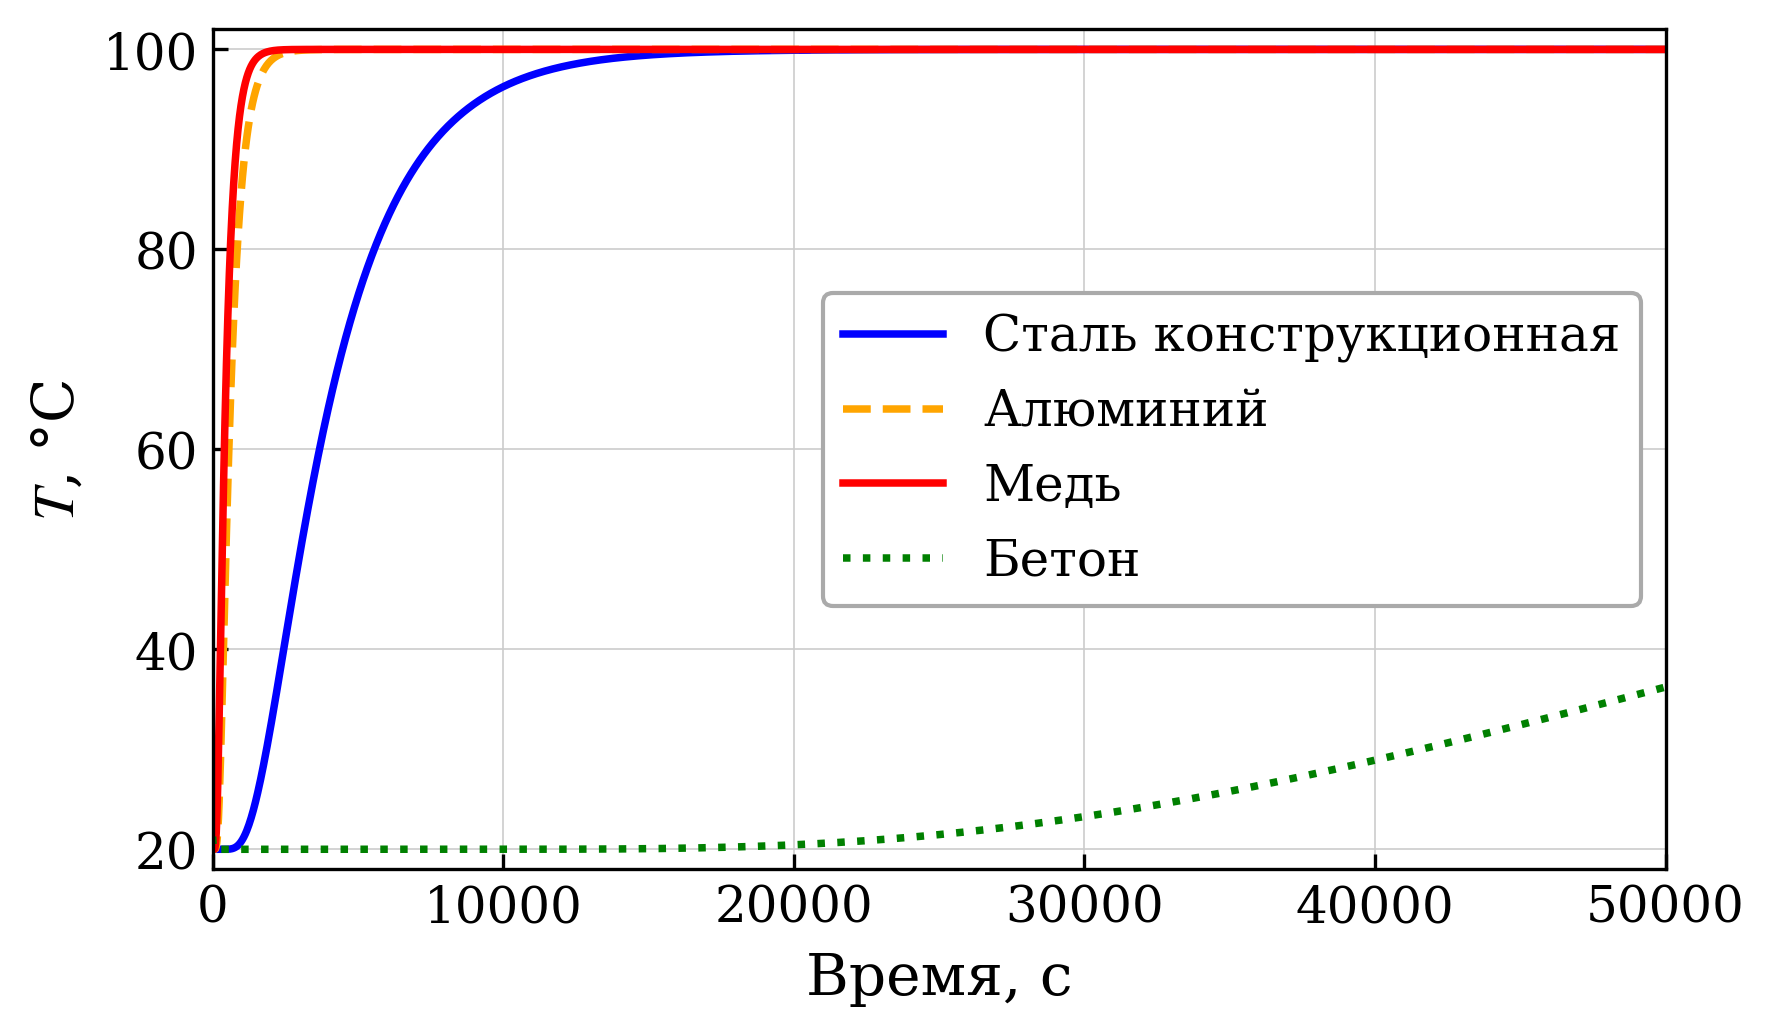
\includegraphics[width=0.9\textwidth]{nir_fig5_materials.png}
    \caption{Динамика прогрева для различных материалов}
    \label{fig:materials}
\end{figure}

Результаты подтверждают, что скорость прогрева определяется 
коэффициентом температуропроводности материала. Медь и алюминий 
достигают равновесного состояния значительно быстрее стали, 
тогда как бетон характеризуется существенно более медленным 
перераспределением тепла.

\subsection{Влияние коэффициента температуропроводности на скорость прогрева}

Анализ результатов показывает, что время достижения температуры 
в центре области, равной $90~\%$ от граничной, обратно 
пропорционально коэффициенту температуропроводности материала. 
Для меди данное время примерно в десять раз меньше, чем для 
конструкционной стали, а для бетона --- примерно в двадцать раз 
больше. 

\section{Исследование влияния граничных условий на распределение температуры}

\subsection{Симметричные граничные условия --- равномерный прогрев}

При задании одинаковой температуры на всех шести гранях
расчётной области тепло распространяется равномерно от
границ к центру тела. В начальный момент времени температура
тела составляет 20 °C, тогда как на всех гранях
поддерживается постоянное граничное значение
 100 °C. Под действием граничных условий фронт
прогрева движется от поверхностей к центру симметрично
по всем трём координатным направлениям, не приобретая
предпочтительной ориентации.

Поскольку граничные условия одинаковы на всех гранях,
поле температур в любой момент времени обладает тройной
симметрией относительно срединных плоскостей $x = L/2$,
$y = L/2$ и $z = L/2$. Данное свойство использовалось
как критерий верификации: значения температуры в
симметрично расположенных узлах расчётной сетки
совпадали с машинной точностью на протяжении всего
расчёта. Проверка подтвердила корректность задания
граничных условий и правильность индексации узлов в
программном модуле.

\subsection{Несимметричные граничные условия и направленный тепловой поток}

При задании различных температур на противоположных
гранях тепловой поток приобретает выраженное направление.
В рамках данного тестового случая на грани $x = 0$
задавалась температура $20$~°C, на грани $x = L$ —
температура $200$~°C, на оставшихся четырёх гранях
поддерживалось значение $100$~°C. Перепад температур
между противоположными гранями составил  180 °C,
что обусловило возникновение направленного потока теплоты
преимущественно вдоль оси~$x$.

В установившемся режиме, когда $\partial T / \partial t = 0$
и внутренние источники теплоты отсутствуют, уравнение
теплопроводности вдоль оси~$x$ в центральной части
тела принимает вид:

\begin{equation}
    \frac{d^2 T}{dx^2} = 0,
    \label{eq:steady_1d}
\end{equation}

\noindent решением которого является линейный профиль температуры.
При подстановке граничных значений аналитическое решение
принимает вид:

\begin{equation}
    T(x) = T_{x^-} + \bigl(T_{x^+} - T_{x^-}\bigr)\cdot x
         = 20 + 180\,x,
    \quad x \in [0;\,1].
    \label{eq:linear_profile}
\end{equation}

Отклонение от линейного закона наблюдается вблизи боковых
граней, где температура $100$~°C создаёт поперечный приток
теплоты в угловых зонах. В центральной части тела влияние
боковых граней пренебрежимо мало, и профиль температуры
близок к аналитическому решению~(\ref{eq:linear_profile}).
Направление вектора теплового потока, определяемого
законом Фурье как $\mathbf{q} = -\lambda\,\nabla T$,
совпадает с направлением убывания температуры и ориентировано
от грани с высокой температурой к грани с низкой, что
соответствует физическому смыслу задачи.

\section{Анализ температурных полей и зон максимального теплового нагрева}

\subsection{Тепловые карты срезов XY и XZ расчётной области}

Пространственное распределение температуры удобно
анализировать посредством двумерных срезов в координатных
плоскостях. Срез в плоскости $z = L/2$ отражает
распределение в плоскости~$XY$, срез в плоскости
$y = L/2$~— в плоскости~$XZ$.

На рисунке~\ref{fig:slices} представлено распределение температуры 
в срединных срезах тела на финальном шаге расчёта. 
Поле практически однородно по всему объёму, что свидетельствует 
о достижении теплового равновесия. 
Незначительный градиент сохраняется лишь в угловых зонах, 
где сходятся три холодные грани.

\begin{figure}[h]
    \centering
    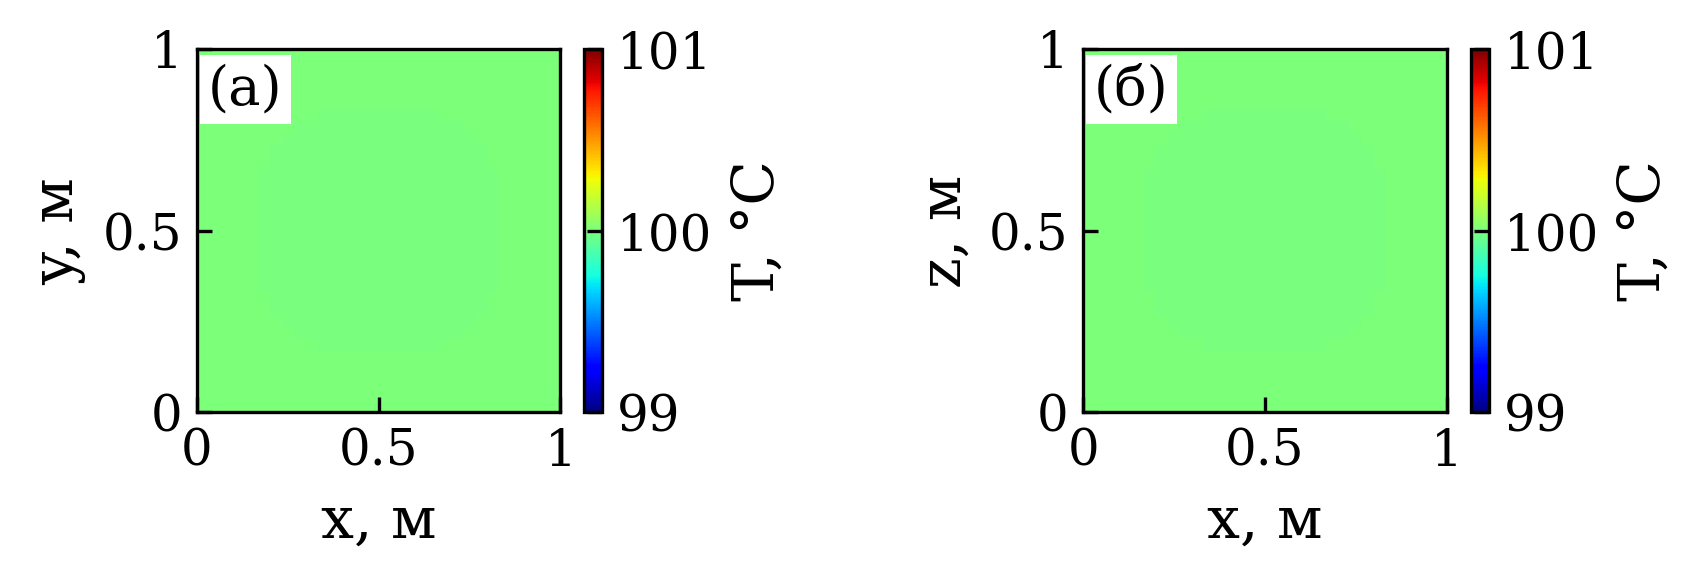
\includegraphics[width=0.9\textwidth]{nir_fig1_slices_2.png}
    \caption{Распределение температуры в срезах плоскостей
             (а)~$XY$ и (б)~$XZ$ при $z = L/2$ и $y = L/2$
             соответственно, финальный шаг расчёта}
    \label{fig:slices}
\end{figure}

При симметричных граничных условиях оба среза
демонстрируют практически однородное поле со
значениями, близкими к $T_\Gamma = 100$~°C.
Незначительная неоднородность сохраняется лишь
в угловых зонах, где сходятся три грани области.


\subsection{Профили температуры вдоль осей и определение зон максимального нагрева}

В начальный
момент профиль вдоль оси~$x$ представляет собой ступенчатую
функцию: во внутренних узлах поддерживается $T_0 = 20$~°C,
тогда как в граничных узлах температура скачкообразно
принимает значение $T_\Gamma = 100$~°C.

На рисунке~\ref{fig:profiles} показаны профили температуры 
вдоль осей $x$ и $y$ в три момента времени. 
На начальном шаге температура внутри тела равна $T_0 = 20~^\circ$С, 
тогда как граничные узлы уже прогреты до $100~^\circ$С. 
По мере протекания процесса профиль выравнивается, 
и к конечному шагу температура по всему объёму достигает граничного значения.

\begin{figure}[h]
    \centering
    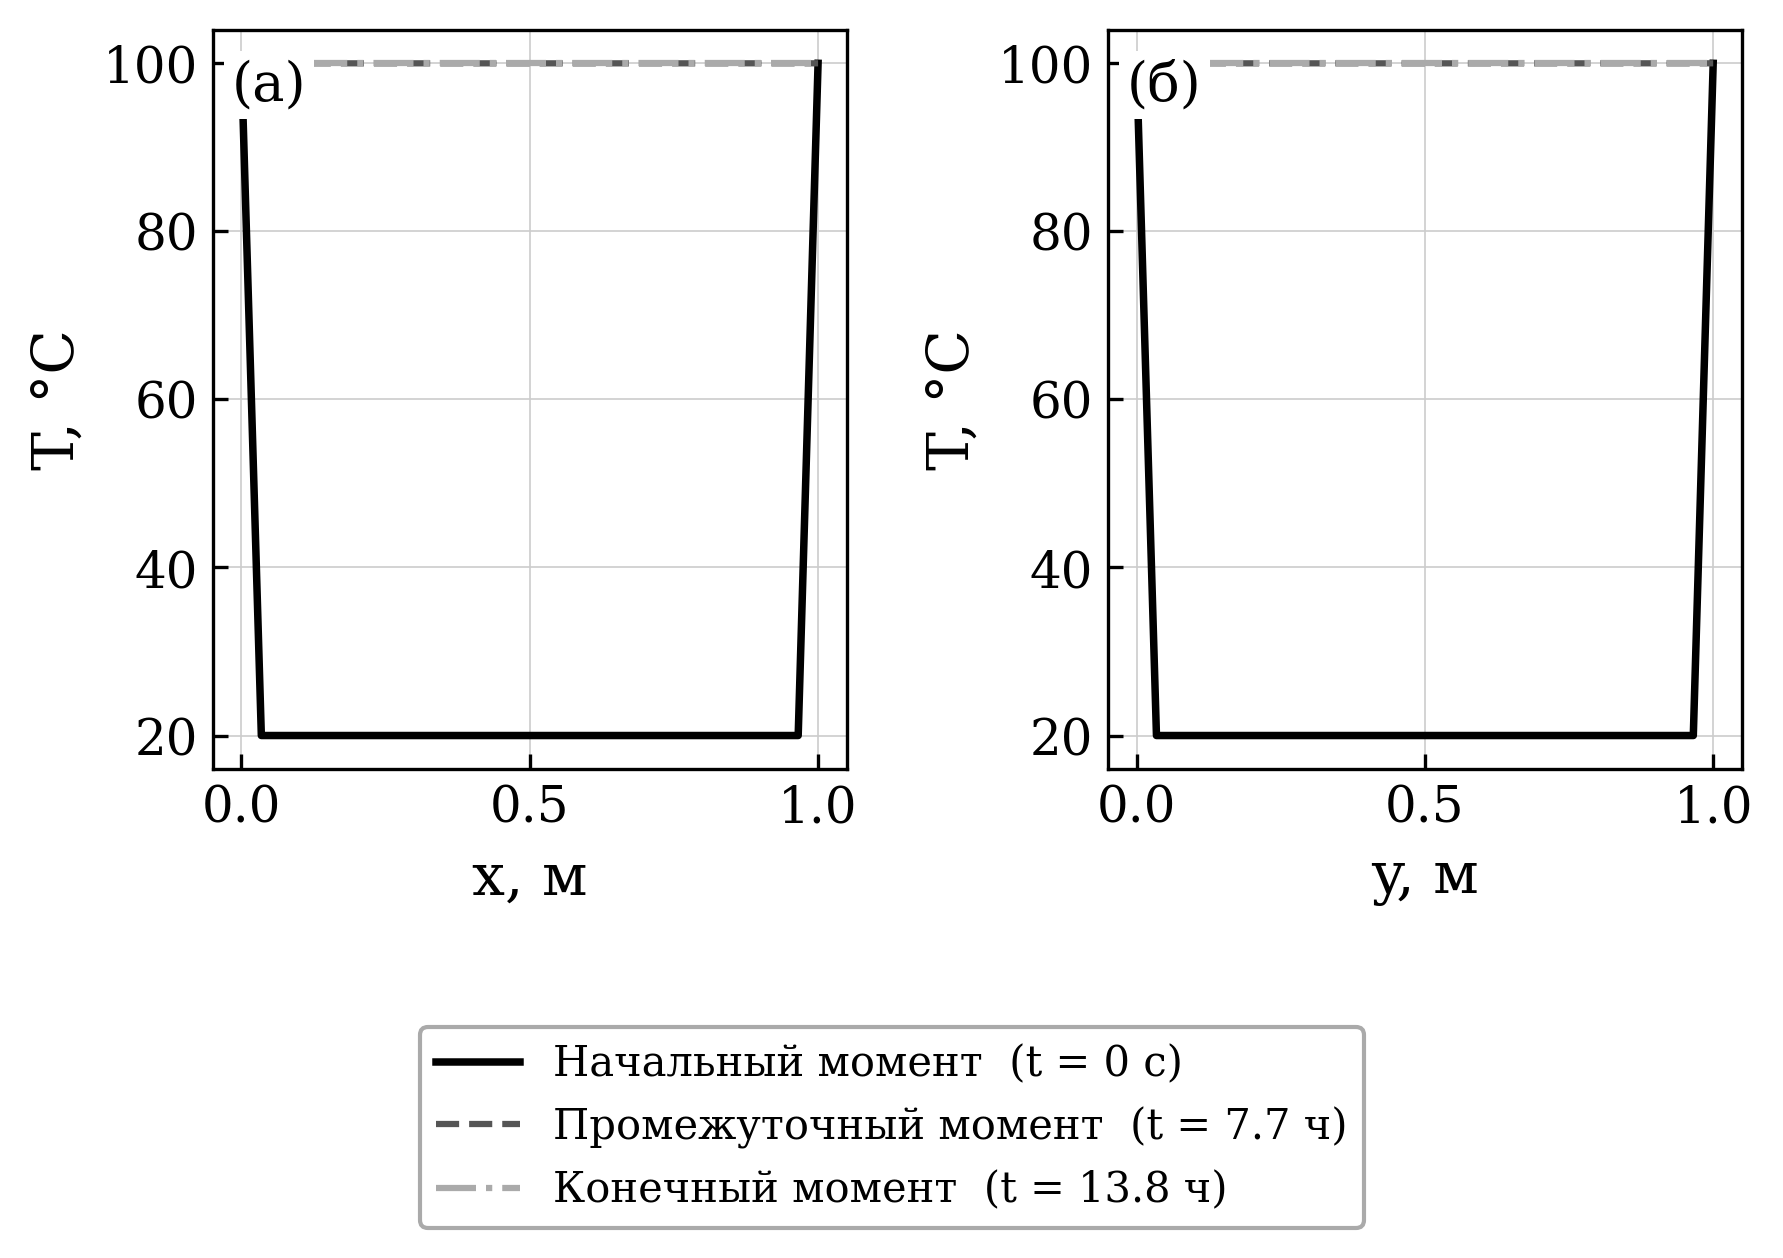
\includegraphics[width=0.9\textwidth]{nir_fig2_profiles_2.png}
    \caption{Профили температуры вдоль осей (а)~$x$ и (б)~$y$
             в начальный, промежуточный и конечный моменты времени}
    \label{fig:profiles}
\end{figure}

В силу симметрии граничных условий профиль по оси~$y$
является зеркальным отражением самого себя относительно
плоскости $y = L/2$. На конечном шаге остаточный перепад
между центром и поверхностью составляет менее $4$~°C,
что свидетельствует о практически полном выравнивании поля.

Зоны максимального нагрева определяются расположением
граней с наибольшей температурой. При симметричных условиях
максимум фиксируется равномерно по всем граням, минимум~—
в центре. При несимметричных условиях зона максимума
смещается в сторону грани с наибольшей температурой.

\section{Сравнение численного и аналитического решений}

Для верификации разработанного программного комплекса выполняется 
сравнение результатов~\cite{чечулин2015качественное} численного моделирования с аналитическим 
решением нестационарной задачи теплопроводности.

\subsection{Аналитическое решение одномерной нестационарной задачи теплопроводности}

Рассматривается одномерная нестационарная задача теплопроводности
\cite{дучков1999тепловой} 
вдоль оси $x$ при следующих условиях: начальная температура 
$T_0 = 20~^\circ$С, температура на грани $x = 0$ равна 
$T_1 = 20~^\circ$С, температура на грани $x = L$ равна 
$T_2 = 100~^\circ$С.

Аналитическое решение данной задачи представляется в виде суперпозиции 
стационарного решения и нестационарной составляющей:
\begin{equation}
    T(x, t) = T_1 + (T_2 - T_1)\frac{x}{L} + 
    \sum_{n=1}^{\infty} B_n \sin\left(\frac{\pi n x}{L}\right) 
    e^{-a\left(\frac{\pi n}{L}\right)^2 t},
\end{equation}
где коэффициенты $B_n$ определяются из начального условия:
\begin{equation}
    B_n = \frac{2}{L} \int_0^L 
    \left[ T_0 - T_1 - (T_2 - T_1)\frac{x}{L} \right] 
    \sin\left(\frac{\pi n x}{L}\right) dx.
\end{equation}

При равномерном начальном распределении $T_0 = \text{const}$ 
коэффициенты принимают вид:
\begin{equation}
    B_n = \frac{2(T_0 - T_1)}{{\pi n}}(-1)^{n+1} - 
    \frac{2(T_2 - T_1)}{\pi n}(-1)^n.
\end{equation}

При $t \to \infty$ нестационарная составляющая затухает и 
распределение температуры стремится к стационарному линейному 
профилю:
\begin{equation}
    T(x) = T_1 + (T_2 - T_1)\frac{x}{L} = 20 + 80x.
\end{equation}

\subsection{Сопоставление численных результатов с аналитическим решением
}

Численное моделирование выполняется в программном комплексе
HeatSim3D со следующими параметрами: материал --- конструкционная
сталь $a = 1{,}28 \cdot 10^{-5}$~м$^2$/с, сетка
$30 \times 30 \times 30$ узлов, $T_0 = 20~^\circ$С,
граничное условие Дирихле $T = 100~^\circ$С на всех гранях,
время моделирования $t_\text{end} = 50000$~с.

Влияние граничных условий на гранях $Y$ и $Z$, заданных 
равными $100~^\circ$С, приводит к отклонению трёхмерного 
численного решения от одномерного аналитического в центральной 
части профиля. Тем не менее характер распределения температуры 
и направление теплового потока качественно совпадают, что 
подтверждает корректность реализованного численного алгоритма.

На рисунке~\ref{fig:verification} представлен профиль температуры вдоль оси~$x$ при $t = 3097$~с. Аналитическое решение получено методом разделения переменных для трёхмерного уравнения теплопроводности. Максимальное отклонение численного решения от аналитического составляет 0,29 °C. Полученная величина погрешности является незначительной по сравнению с общим диапазоном изменения температуры, что свидетельствует о высокой точности численного метода. Наблюдаемое совпадение кривых подтверждает адекватность выбранной расчётной схемы и корректность реализации алгоритма.
\begin{figure}[h]
    \centering
    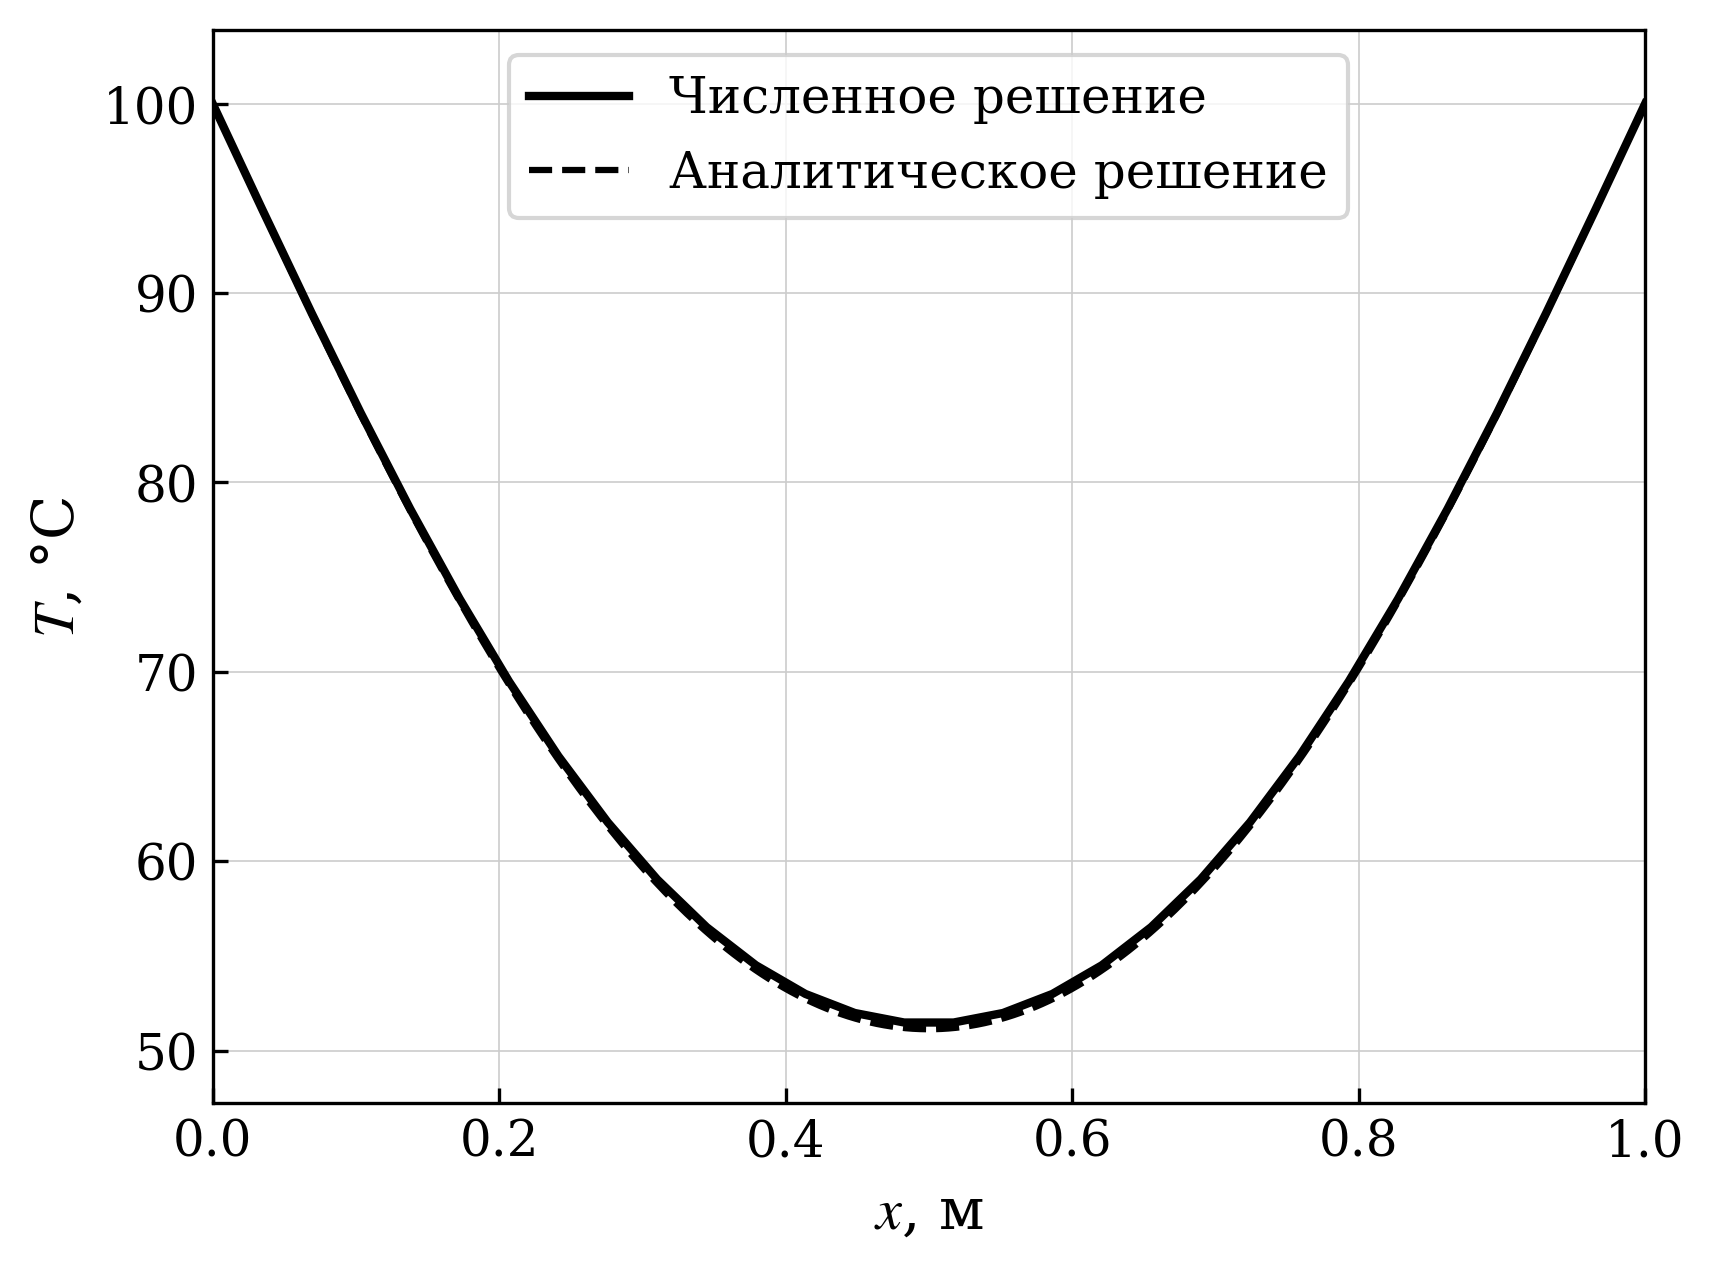
\includegraphics[width=0.9\textwidth]{nir_verification.png}
    \caption{Профиль температуры $T(x)$ при $y = z = L/2$,
             $t = 3097$~с. Сплошная линия --- численное решение,
             штриховая --- аналитическое}
    \label{fig:verification}
\end{figure}

Проведённые расчёты подтвердили соответствие результатов теоретическим оценкам и корректность работы численной схемы. Программный комплекс HeatSim3D пригоден для решения практических задач теплопроводности для различных конструкционных материалов.